 \makeatletter
\cxset{plain sections/.style={
 chapter name = CHAPTER,
 chapter toc = true,
 chapter color= thegray,
 chapter opening = right, 
 chapter numbering = arabic,
 chapter font-family= sffamily,
 chapter font-weight= bold,
 chapter font-size= LARGE,
 chapter before={\thinrule\vspace*{20pt}\par\hfill\hfill},
 chapter after={\vskip0pt\par},
 chapter spaceout = soul,
 number font-size= Large,
 number font-family= rmfamily,
 number font-weight= bfseries,
 number color=thegray,
 number before=\vspace*{5pt}\hfill\hfill,
 number dot=.,
 number after={\hspace*{7pt}\par},
 title beforeskip={\vspace*{10pt}},
 title afterskip={\vspace*{50pt}\par},
 title before={\hfill\hfill\raggedleft},
 title after={\par\thinrule},
 title font-family=\sffamily,
 title font-color= teal,
 title font-weight=\bfseries,
 title font-family=\sffamily,
 title font-size= Large,
 title font-shape= upshape,
 title spaceout= none,
 title beforeskip={\vspace*{10pt}},
 title afterskip={\vspace*{50pt}\par},
 title before={\hfill\hfill\raggedleft},
%
% numbers
% number font-family=\sffamily,
% number font-weight=\bfseries,
 number color=thelightgray,
 number before=\par\vspace*{5pt}\hfill\hfill,
 number dot=,
 number after={\hspace*{7pt}\par},
 number position=rightname,
 section color= thered,     
 section beforeskip=15pt,
 section afterskip=15pt,
 section indent=0pt,
 section font-family= sffamily,
 section font-size= LARGE,
 section font-weight= bfseries,
 section font-shape=,
 section align= centering,
 section numbering prefix =,%use \thechapter. for books or add as option
 section numbering= arabic,
 section spaceout=none,
 section number after=ooo,
 subsection color= thered,
       subsection beforeskip=10pt,
       subsection afterskip=10pt,
       subsection indent=0pt,
       subsection font-family= rmfamily,
       subsection font-size= large,
       subsection font-weight= bold,
       subsection font-shape= upshape,
       subsection align= centering,
       subsection numbering prefix=\thesection.,%\S\hairsp,%add . 
       subsection numbering custom =\@arabic\c@subsection,% \two@digits{\@arabic\c@subsection},%
       subsubsection color= gray,
       subsubsection beforeskip=5pt plus3pt minus 2pt,
       subsubsection afterskip=5pt,
       subsubsection indent=0pt,
       subsubsection font-family= rmfamily,
       subsubsection font-size= normalfont,
       subsubsection font-weight= bold,
       subsubsection font-shape= itshape,
       subsubsection align= centering,
       subsubsection numbering prefix =\thesubsection.\@arabic\c@subsubsection,
       subsubsection numbering custom =, %\two@digits{\@arabic\c@subsubsection},
       subsubsection number after =, 
%
       paragraph color= thegrey,
       paragraph beforeskip=,
       paragraph afterskip=-0.5em,
       paragraph indent=0pt,
       paragraph font-family= rmfamily,
       paragraph font-size= large,
       paragraph font-weight= bfseries,
       paragraph font-shape=,
       paragraph align= centering,
       paragraph number after = 0pt,
       paragraph numbering=numeric,
       subparagraph color= thered,
       subparagraph beforeskip=0pt,
       subparagraph afterskip=-.5em,
       subparagraph indent=0pt,
       subparagraph font-family= sffamily,
       subparagraph font-size= large,
       subparagraph font-weight= normalfont,
       subparagraph font-shape= slshape,
       subparagraph align= RaggedRight,
       subparagraph number after =, % can affect all needs checking
       %subsubsection numbering prefix=\S\hairsp\thesection,%add . here if need be
       subparagraph numbering=none,
}
}
\cxset{plain sections}
\cxset{style13/.style={
 name= {\protect\pan अमुकग्रन्थे},
 chapter spaceout = none,
 numbering=arabic,
 number font-size= HUGE,
 number font-family= sffamily,
 number font-weight= bfseries,
 number color= gray!50,
 number before=\par\vspace*{5pt}\hfill\hfill,
 number dot=,
 number after={\hspace*{7pt}\par},
 number position=rightname,
 chapter font-family= sffamily,
 chapter font-weight= bold,
 chapter font-size= LARGE,
 chapter before={\tikzrule\vspace*{20pt}\par\hfill\hfill},
 chapter color= black!50,
 title beforeskip={\vspace*{10pt}},
 title afterskip={\vspace*{50pt}\par},
 title before={\hfill\hfill\raggedleft},
 chapter rule color=teal,
 title after=\par\tikzrule,
 title font-family= sffamily,
 title font-color= teal,
 title font-weight= bfseries,
 title font-size= huge,
 section indent=-1em,
 section align= left,
 section numbering= arabic,
 section indent=0pt,
 section beforeskip=0pt,
 section afterskip= 10pt,
 section color=teal,
 subsection align= ,
 subsection font-family= sffamily,
 subsection font-weight= bfseries,
 subsection color = teal,
 subsection font-size= large,
 subsection font-shape=,
 subparagraph number after=,
 subsubsection align=,
}
}
\cxset{style13}

\renewparagraph
\renewsection
\renewsubsection
\renewsubparagraph
\renewsubsubsection

\makeatother
  
 \cxset{style29/.style={
 name={},
 numbering=arabic,
 number font-size=normalsize,
 number font-family=sffamily,
 number font-weight=bfseries,
 number before={\vspace*{30pt}},
 number position=leftname,
 number after=\hrule width\textwidth height1pt\par,
 chapter font-family=sffamily,
 chapter font-weight=,
 chapter font-size=small,
 chapter before={\vskip2.5pt},
 chapter after=,
 chapter color= black!90,
 number color= black!90,
 title beforeskip={},
 title afterskip={\bigskip},
 title before=,
 title after={\par},
 title font-family=rmfamily,
 title font-color= black!80,
 title font-weight=bfseries,
 title font-size=\huge,
 chapter title align=raggedright,
 section indent=0pt,
 section numbering=arabic,
 section font-family=\rmfamily,
 section font-shape=\upshape,
 section numbering prefix=\thechapter.,
section numbering suffix=,
 section color=black,
 subsection number after=\quad,
 subsection number after=\quad}}
\cxset{style29}

\endinput
\renewsection\renewsubsection

\chapter{Reading Systems: An Introduction to Digital Document Processing}
\bigskip\bigskip

\textit{Lambert Schoemacher}
\bigskip\bigskip\bigskip\bigskip

\section{Introduction}

Style 29 comes from the computer world and is representative of conference publications. It is always instructive
to go back and read research undertaken decades ago to understand the present state of the art but also to study how standards emerge and the competitive forces that shape the survivability of computer software. 


\begin{figure}[ht]
\centering
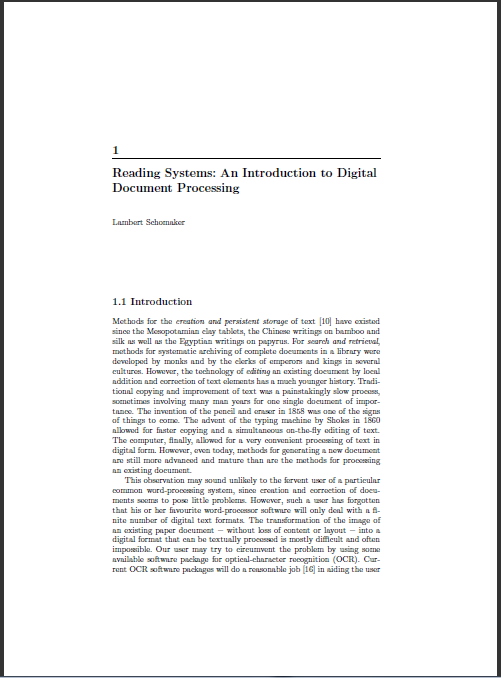
\includegraphics[width=0.5\textwidth]{./chapters/chapter29.png}
\end{figure}

The template is based on a Springer-Verlag London publication dated 2007 from a series on Advance Pattern Recognition. Many of these publications were prepared using \latex itself and templates from this firm are still available and on ctan for its many journals. The introduction by Schoemacher provides background information to anyone interested to understand the evolution of document processing. 

\section{Documents}

The word document comes from the Latin word ‘documentum’, which has the same
stem as the verb ‘doceo’ (meaning ‘to teach’), plus the suffix ‘-umentum’ (indicating
a means for doing something). Hence, it is intended to denote ‘a means for teaching’
(in the same way as ‘instrument’ denotes a means to build, ‘monument’ denotes a
means to warn, etc.). Dictionary definitions of a document are the following [2]:
\begin{enumerate}
\item Proof, Evidence
\item An original or official paper relied on as basis, proof or support of something
\item Something (as a photograph or a recording) that serves as evidence or proof
\item A writing conveying information
\item A material substance (as a coin or stone) having on it a representation of thoughts
by means of some conventional mark or symbol.
\end{enumerate}

The first definition is more general. The second one catches the most intuitive
association of a document to a paper support, while the third one extends the definition
to all other kinds of support that may have the same function. While all
these definitions mainly focus on the bureaucratic, administrative or juridic aspects
of documents, the fourth and fifth ones are more interested in its role of information
bearer that can be exploited for study, research, information. Again, the former
covers the classical meaning of documents as written papers, while the latter extends
it to any kind of support and representation. Summing up, three aspects can be
considered as relevant in identifying a document: its original meaning is captured
by definitions 4 and 5, while definition 1 extends it to underline its importance as
a proof of something, and definitions 2 and 3 in some way formally recognize this
role in the social establishment.

\section {Current Landscape}

While up to recently documents were produced in paper format, and their digital
counterpart was just a possible consequence carried out for specific purposes,
nowadays we face the opposite situation: nearly all documents are produced and
exchanged in digital format, and their transposition on a tangible, human-readable
support has become a successive, in many cases optional, step. Additionally, significant
efforts have been spent in the digitization of previously existing documents


\section{The Shelf-life of Documents}

In a post at \texttt{TX.SX} Barbara Beeton mentioned that one of the advantages of \tex is that documents produced by it results in documents with a very long shelf life and that Mathematics has a long shelf life.
Of course the best way to ensure a long shelf life is to have the document printed out and stored in an archive.
Paper is still the best way to ensure long term survivability. Knuth’s idea when he insisted that \tex cannot be changed was to ensure that a document could be printed always the same way. I am not too sure if this is an absolute necessity, as what is important is for the content to survive.

